% How to Draw Carnot Cycle in TikZ
% Latexdraw.com
% 15/02/2021, 21:45

\documentclass [border = .2cm] {standalone}

\usepackage{tikz}
% For "Arrowhead in a midlle of a line"
\usetikzlibrary{decorations.markings}

\begin{document}

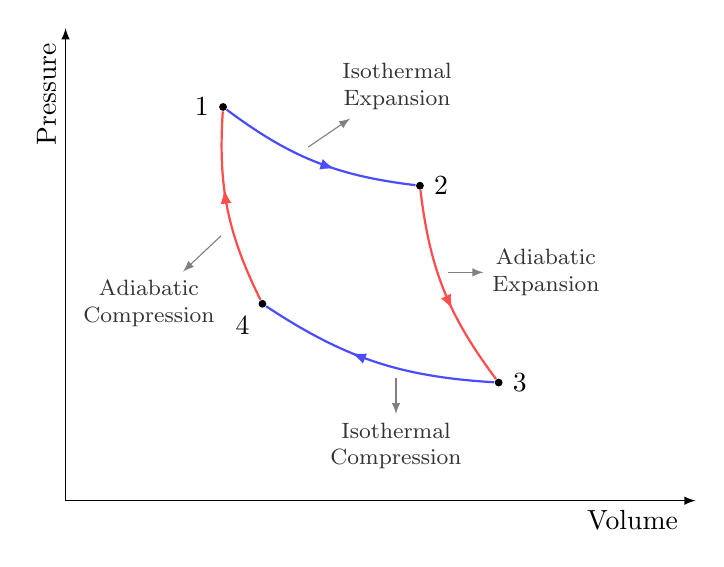
\begin{tikzpicture}
[
% Corner style
	corner/.style={ 
		circle,
		fill,	
		inner sep=1pt},
% Line with Arrow style
	arrowline/.style={
		thick,
		postaction = decorate,
		decoration = {markings,
			mark = at position .6 with \arrow{latex}
		}
	},
% Pin style
	every pin/.style = {
		black!80, 
		inner sep = 1mm, 
		align = center,
		font = \footnotesize, 
		pin edge = {-latex, thin, line to}},
]

% Draw axis with labels
\draw [latex-latex] (0,6)  |- (8,0) 
	node [pos=.95,below] {Volume}
	node [pos=0.07,above,rotate=90] {Pressure};

% Cycle corners
\node[corner,
	label = {left:$1$}] (1) at (2,5){} ;

\node[corner,
	label = {right:$2$}] (2) at (4.5,4){} ;

\node[corner,
	label = {right:$3$}] (3) at (5.5,1.5){} ;

\node[corner,
	label = {below left:$4$}] (4) at (2.5,2.5){} ;

% Curved lines
\draw [arrowline,blue!70] (1) to [bend right = 15] 
	node [pos = .4, pin = {45:Isothermal\\Expansion}] {} (2);

\draw [arrowline,red!70 ] (2) to [bend right = 15] 
	node [pos = .4, pin = {right:Adiabatic\\Expansion}] {}(3);

\draw [arrowline,blue!70] (3) to [bend left  = 15] 
	node [pos = .4, pin = {below:Isothermal\\Compression}] {} (4);

\draw [arrowline,red!70 ] (4) to [bend left  = 15] 
	node [pos = .4, pin = {260:Adiabatic\\Compression}] {} (1);

\end{tikzpicture}

\end{document}